%!TEX TS-program = xelatex
%!TEX encoding = UTF-8 Unicode

Antes de comenzar el análisis correspondiente a los distintos estadios de sueño, vamos mostrar una serie de gráficos y medidas de centralidad que obtuvimos como consecuencia de calcular los promedios de todas las matrices por cada fase N1, N2, N3 y W.

Lo primero que obtuvimos fue un grafo pesado completo para cada fase. En este caso las aristas dibujadas no está en proporción a su peso ya que no podría apreciarse en este tipo de gráfico.

\begin{figure}[H]
    \centering
    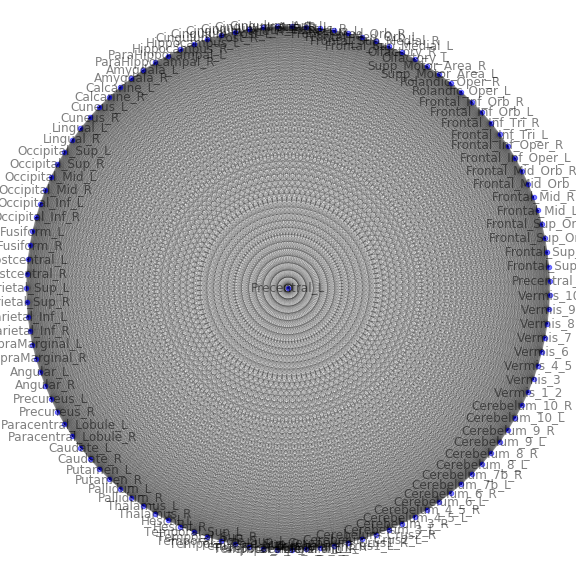
\includegraphics[width = 4in]{img/avg_w.png}
    \caption{Red del estadio W}
    \label{fig:avg-w}
\end{figure}

\begin{figure}[H]
    \centering
    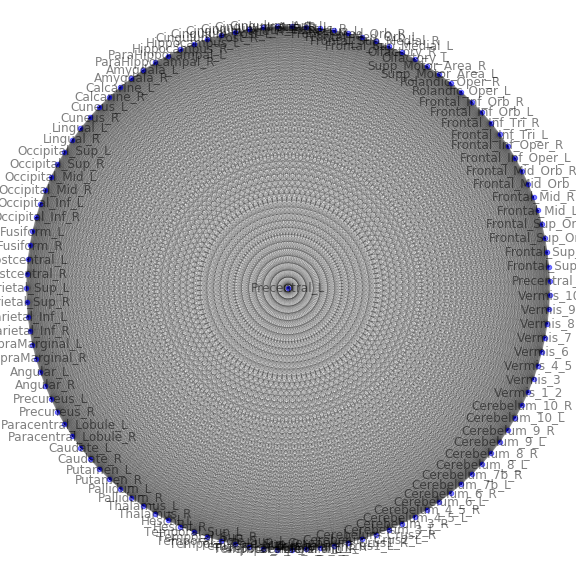
\includegraphics[width = 4in]{img/avg_n1.png}
    \caption{Red del estadio N1}
    \label{fig:avg-n1}
\end{figure}

\begin{figure}[H]
    \centering
    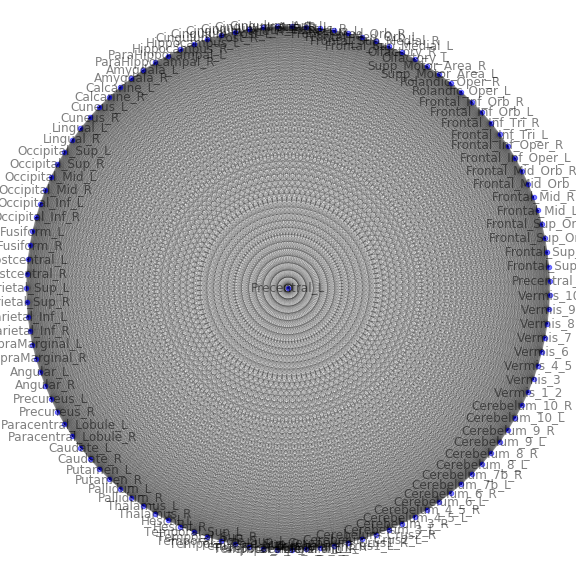
\includegraphics[width = 4in]{img/avg_n2.png}
    \caption{Red del estadio N2}
    \label{fig:avg-n2}
\end{figure}

\begin{figure}[H]
    \centering
    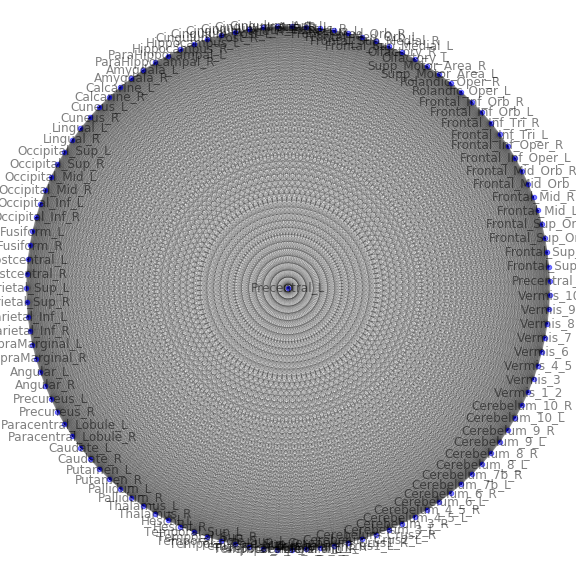
\includegraphics[width = 4in]{img/avg_n3.png}
    \caption{Red del estadio N3}
    \label{fig:avg-n3}
\end{figure}

Como mencionamos en el párrafo anterior, son grafos completos y en esta primera visualización no podemos extraer más información.

\subsection{Medidas de centralidad}
A continuación vamos a calcular algunas medidas de centralidad no para los grafos originales ya mencionados, sino sobre la transformación de los mismos a grafos no pesados y posteriormente tomando para de ellos subconjuntos de subgrafos en función de densidades previamente elegidas.

\begin{figure}[H]
    \centering
    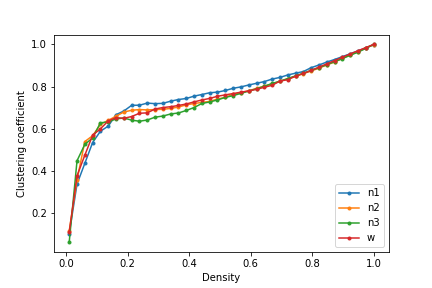
\includegraphics[width = 6in]{img/clust_coeff.png}
    \caption{Coeficiente de clustering}
    \label{fig:clust-coef}
\end{figure}

Se puede ver un crecimiento muy acelerado del coeficiente de clustering para los grafos de hasta una densidad de 0.2 del total de aristas, luego tal umbral el crecimiento se estanca y hasta disminuye para la fase \textbf{N3} pero la tendencia es en crecimiento pero con una pendiente muy pequeña.

\begin{figure}[H]
    \centering
    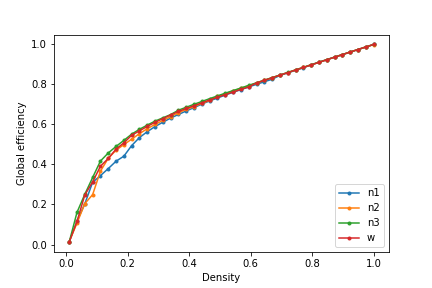
\includegraphics[width = 6in]{img/efficiency.png}
    \caption{Eficiencia}
    \label{fig:efficiency}
\end{figure}

Como para muchas de las densidades utilizadas se obtienen grafos que no son conexos, en lugar de usar el camino mínimo como medida de centralidad, utilizamos la medida de eficiencia global. La tendencia de las fases de sueño es creciente similar a una función logarítmica, salvo por \textbf{N1} que en todo momento se encuentra por debajo de las demás fases.

\begin{figure}[H]
    \centering
    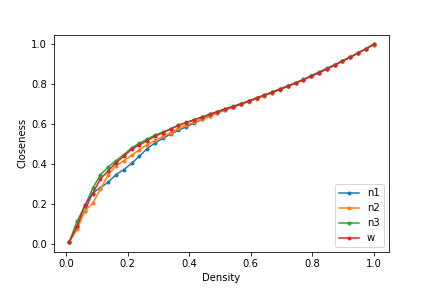
\includegraphics[width = 6in]{img/closeness.png}
    \caption{Cercanía}
    \label{fig:closeness}
\end{figure}

La medida de centralidad de cercanía también parece crecer muy rápidamente para las primeras densidades y luego el mismo crece casi linealmente.

\begin{figure}[H]
    \centering
    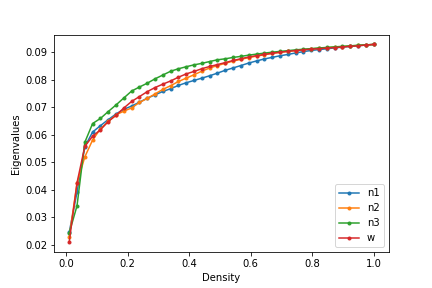
\includegraphics[width = 6in]{img/eigenvector.png}
    \caption{Autovalores}
    \label{fig:eigen}
\end{figure}

Para terminar observamos la medida de autovalores para las distintas densidades y se aprecia que también en las primeras densidades aumenta muy rápidamente y luego continúa el crecimiento pero con una acelaración mucho menor.

\begin{figure}[H]
    \centering
    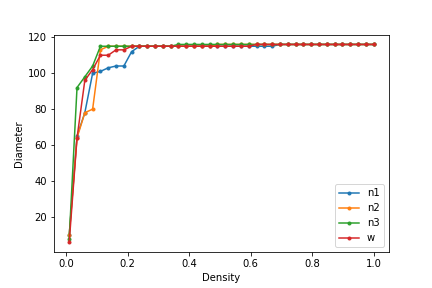
\includegraphics[width = 6in]{img/diameter.png}
    \caption{Diámetro}
    \label{fig:diameter}
\end{figure}

Para terminar calculamos el diámetro para las distintas densidades, como en algunos cortes se obtienen grafos no conexos, en esos casos decidimos graficar el máximo de los diámetros todas las componentes conexas de cada grafo. Aproximadamente se puede ver que ya para una densidad cercana al 0.3, se obtienen grafos fuertemente conectados \textbf{N2} y \textbf{N3} y para \textbf{N1} y \textbf{W} con menos de 3 componentes conexas. Como puede verse ya para la densidad de 0.7 todas las fases del sueño presentan un grafo fuertemente conexo.

\subsection{Visualización de comunidades}
Elegimos 4 densidades para visualizar como se agrupan los nodos de acuerdo a sus conexiones.

\begin{figure}[H]
    \centering
    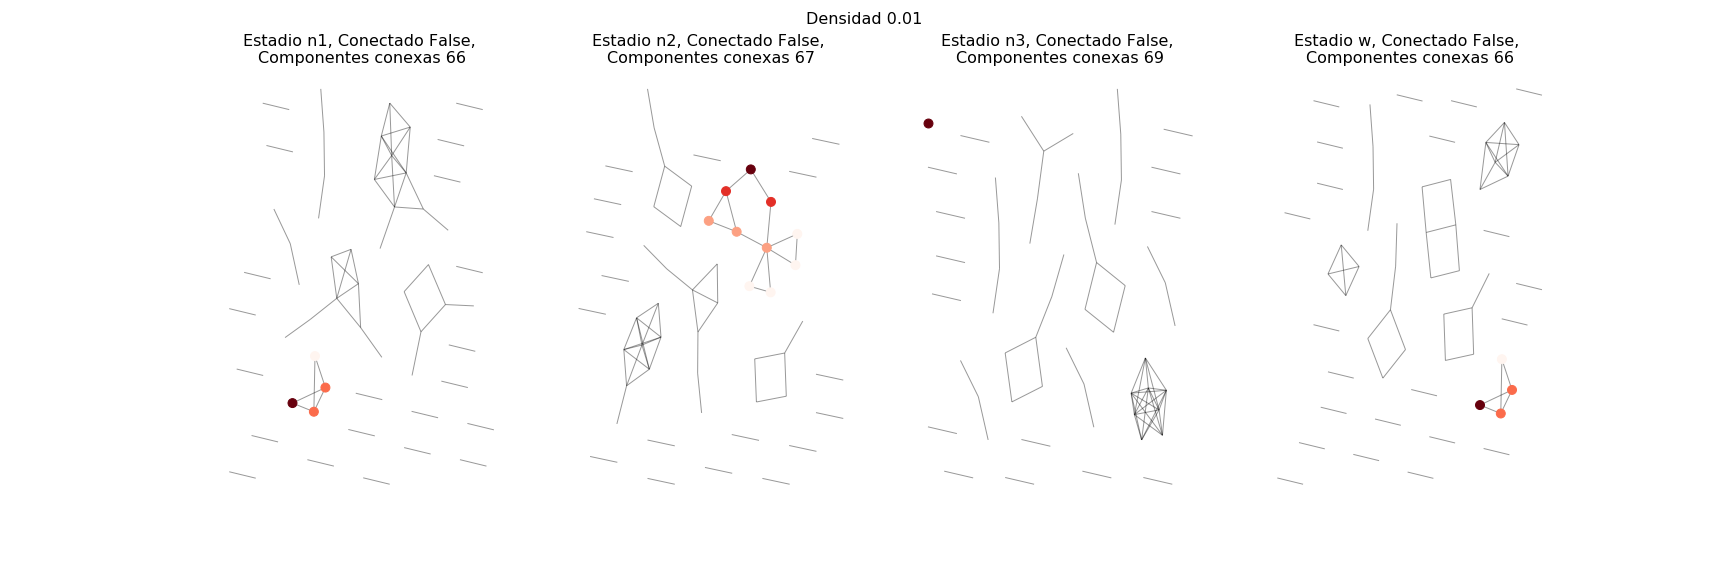
\includegraphics[width = \textwidth]{img/unweight_graphs_001.png}
    \caption{Estadios para densidad 0.01}
    \label{fig:unweight-001}
\end{figure}

En este caso se ve como todos los estadios tienen muchas componentes conexas y poca conexión entre ellas mismas.

\begin{figure}[H]
    \centering
    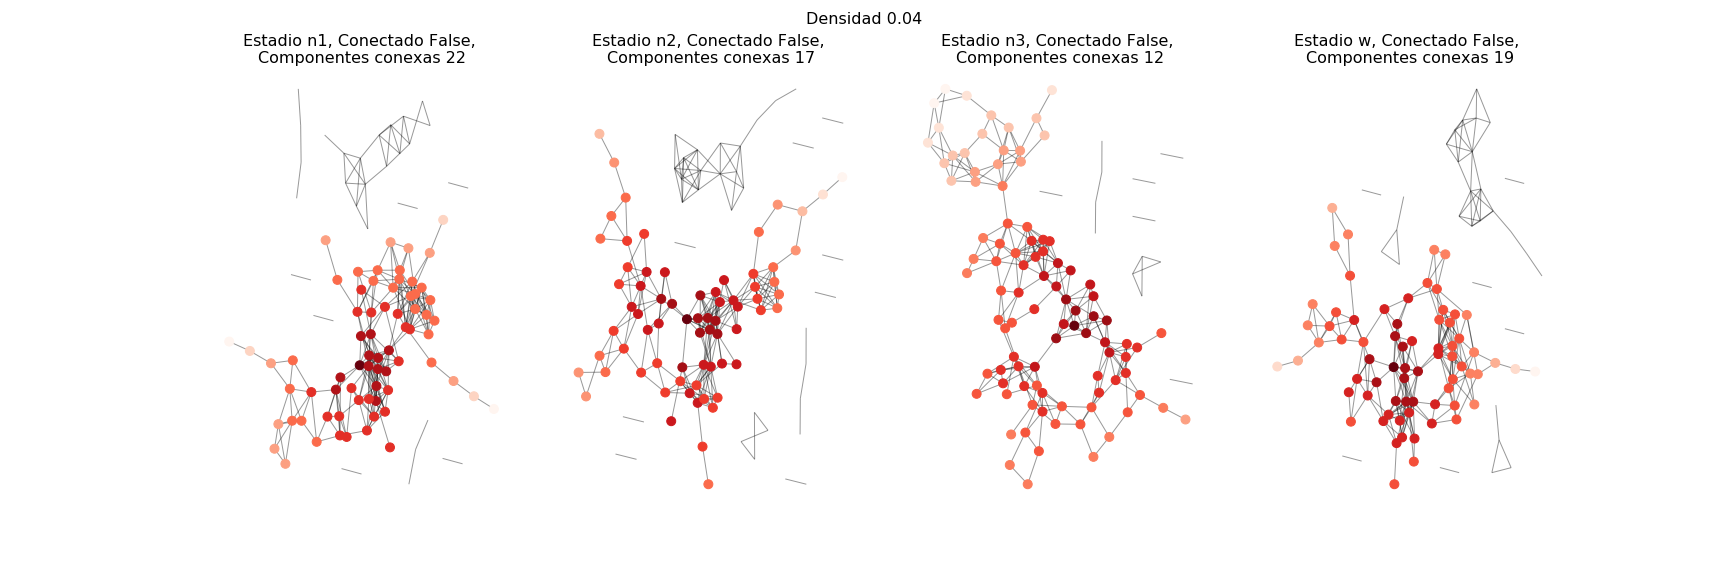
\includegraphics[width = \textwidth]{img/unweight_graphs_004.png}
    \caption{Estadios para densidad 0.04}
    \label{fig:unweight-004}
\end{figure}

Ya en esta etapa se ve que los nodos están mucho mas relacionados entre sí y la fase \textbf{N3} es la más conectada.
\begin{figure}[H]
    \centering
    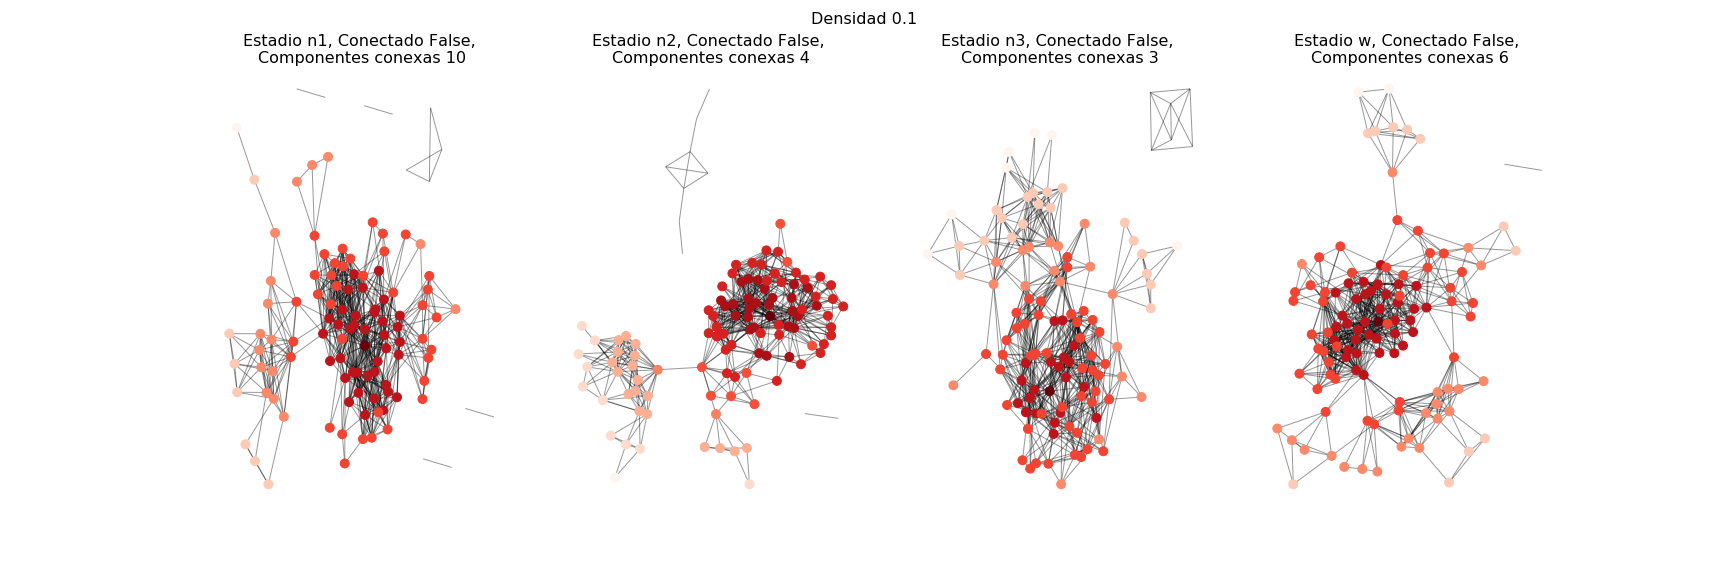
\includegraphics[width = \textwidth]{img/unweight_graphs_01.png}
    \caption{Estadios para densidad 0.1}
    \label{fig:unweight-01}
\end{figure}

En este corte solo el estadio \textbf{N1} tiene más de 10 componentes conexas, en cambio para \textbf{N2}, \textbf{N3} y \textbf{W} se observan grandes comunidades conectadas por algunas aristas entre ellas.

\begin{figure}[H]
    \centering
    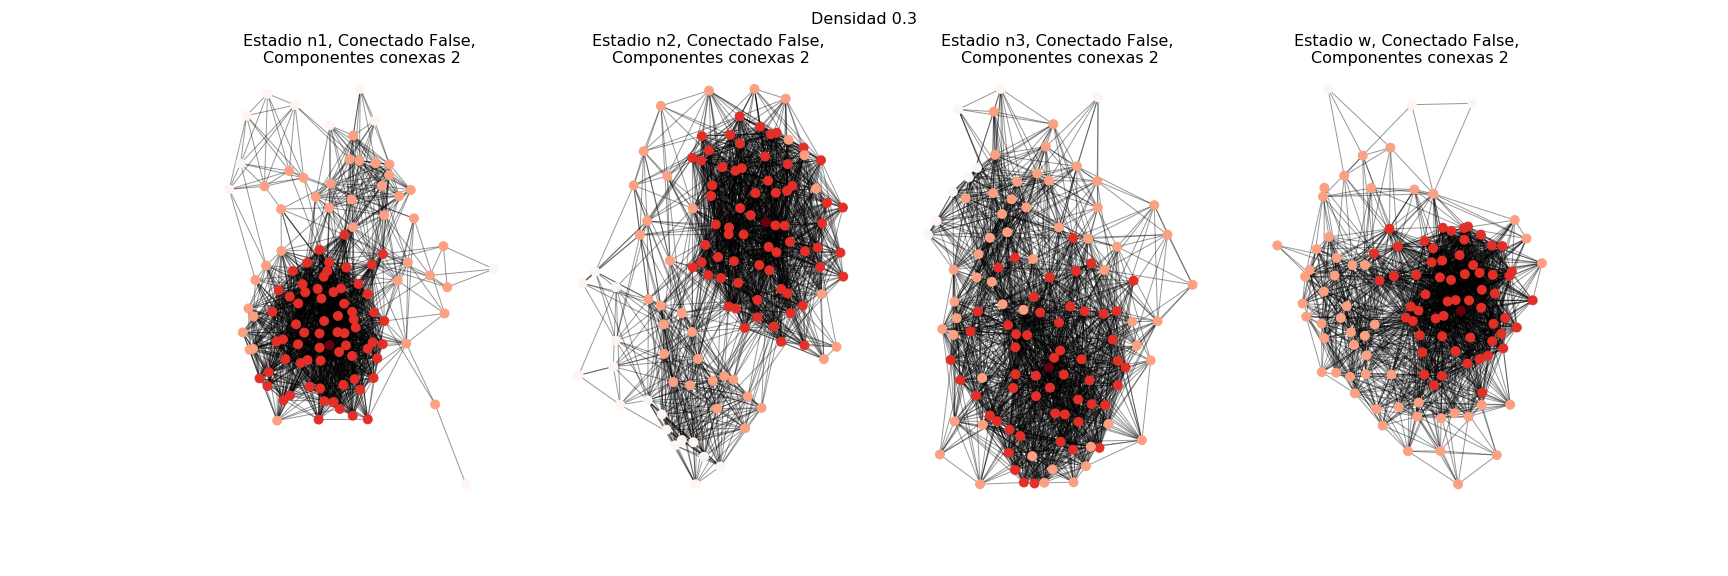
\includegraphics[width = \textwidth]{img/unweight_graphs_03.png}
    \caption{Estadios para densidad 0.3}
    \label{fig:unweight-03}
\end{figure}

Para finalizar en esta última densidad elegida, se puede observar que en todos los estadios el nodo asilado es el mismo el número 115, en \textbf{N3} se puede apreciar un único agrupamiento de nodos, en \textbf{N2} se ven dos grupos definidos y conectados entre ellos, mientras que en \textbf{N1} y \textbf{W} se observa un gran grupo conectado con otros más pequeños.